% !TeX encoding = UTF-8
% !TeX program = lualatex
% !TeX spellcheck = en_US
% !TeX root = thesis.tex

\chapter{Implementation of ventilation metrics}
\label{chap:OF_custom_features}
\index{OpenFOAM!metrics}

This chapter will introduce the software \gls{OpenFOAM} while also giving an overview of metrics that will be used to assess \gls{NVP}.




\section{Indoor air quality}
%\section{Metrics for natural ventilation potential}


Ventilation of buildings is not only an energy-related concern involving heating or cooling a space, it also relates to the well-being of its occupants.

Studies have shown that high CO$_2$ levels impair occupants' ability to focus \citep{Heath2002,Kosonen2004}. This is a worthwhile concern for residential buildings, but also for schools and offices. Good \NVP\ can help keep CO$_2$ concentration below harmful levels.
 

%a student's learning ability. A reasonably low CO$_2$ level is necessary  also in office environments in order to prevent a negative influence on the performance of the working occupants 

\NVP\ can be measured by different metrics, three of which are discussed below:

\begin{enumerate}
\item The \textit{\ACR}\ is a metric that estimates an average change of air in a room depending on the flow-rate inwards and outwards. Thus, it is a metric unable to describe air flow patterns inside the room. It is, however, used as a metric in many guidelines \citep{Limb1995, Humphreys2006}.

\item The \textit{age of air} is another commonly used measure. It describes the amount of time it takes for an air particle to reach a certain point in the space with respect to a reference position. The metric relies on the assumption that the age of the air is independent of the local distribution of emission sources. Thus, it represents an appropriate method for comparing different ventilation systems \citep{SHERMAN2007}.

\item The \textit{CO$_2$ concentration} in a space compared to the outdoor \textit{CO$_2$ concentration} is often used to assess the performance of a building ventilation system. It is used in various standards. This stems from studies by Max Joseph von Pettenkofer who, in the late 19th century, proposed that the CO$_2$ concentration should not exceed \SI{1000}{ppm} in order to maintain a hygienic indoor air quality.
\end{enumerate}


There are other metrics used to assess \NVP\ such as the ventilation effectiveness and efficiency which evaluate a tracer concentration to determine \ACR s. In the interest of time, these are not considered in this thesis.








\begin{figure}
	\subfloat[][]%
	{\includegraphics[width=.346\textwidth, trim= 15cm 5.5cm 12.5cm 5cm, clip]{images/AoA/geometry_room_2}\hfill
		\begin{tikzpicture}[scale=1.5]
		\begin{scope}[overlay]
		\draw [->] (-3.1,0) -- (-2.8,0) node [below] {$x$};
		\draw [->] (-3.1,0) -- (-3.1,0.3) node [left] {$y$};
		\end{scope}			
		\end{tikzpicture}}\hfil
	\subfloat[][]%
	{\includegraphics[width=.31\textwidth, trim= 25cm 3.5cm 27.5cm 18cm, clip]{images/AoA/topview_magU_1_5m_glyph_3}}\hfil
	\subfloat[][]%
	{\includegraphics[width=.343\textwidth, trim= 27.5cm 15cm 32.5cm 18cm, clip]{images/AoA/topview_glyph_2D.png}}\hfil	\\
	%	\includegraphics[scale=.05, trim= 72cm 165cm 77cm 20cm, clip]{images/AoA/topview_Aoa_025m}
	\vspace*{0.4cm}
	\includegraphics[width=.55\textwidth, trim= 32.5cm 80cm 25cm 8.5cm, clip]{images/AoA/topview_magU_1_5m_glyph_3}\\
	\subfloat[][]%
	{\includegraphics[width=.33\textwidth, trim= 31cm 12.5cm 35cm 17.5cm, clip]{images/AoA/topview_streamlines_10m_magU_left.png}}\hfil	
	\subfloat[][]%
	{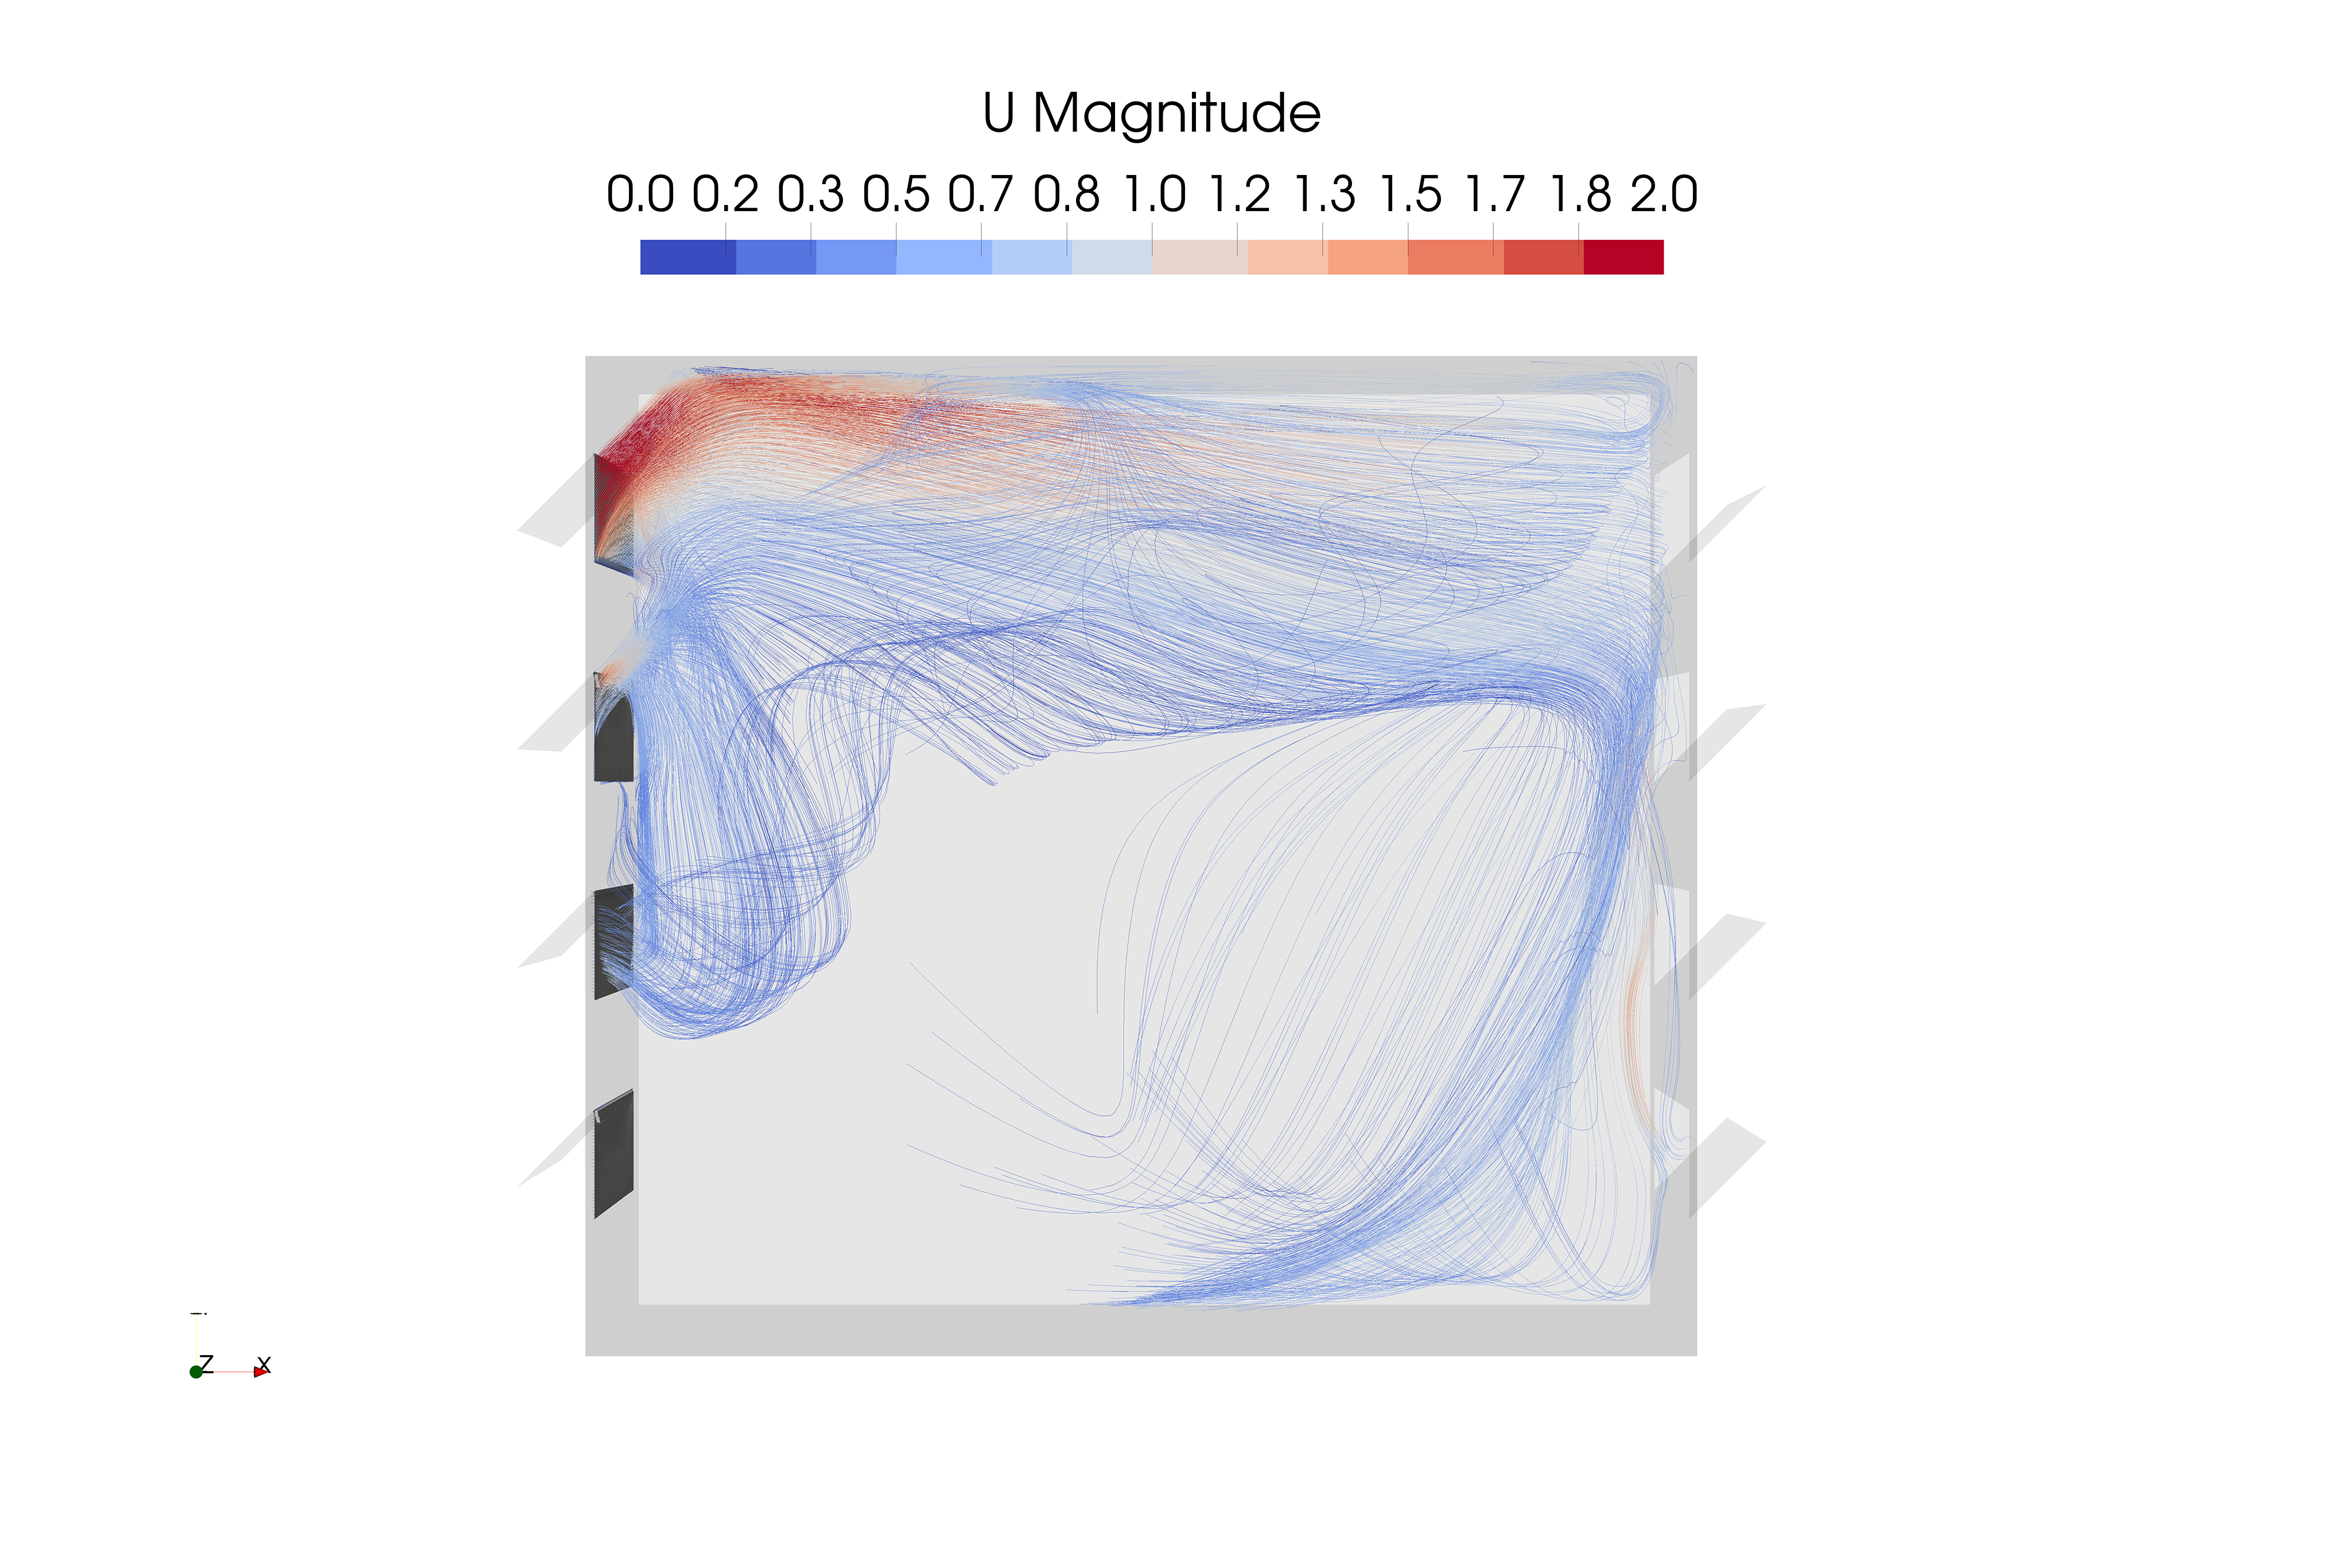
\includegraphics[width=.33\textwidth, trim= 31cm 12.5cm 35cm 17.5cm, clip]{images/AoA/topview_streamlines_20m_magU_left.png}}\hfil	
	\subfloat[][]%
	{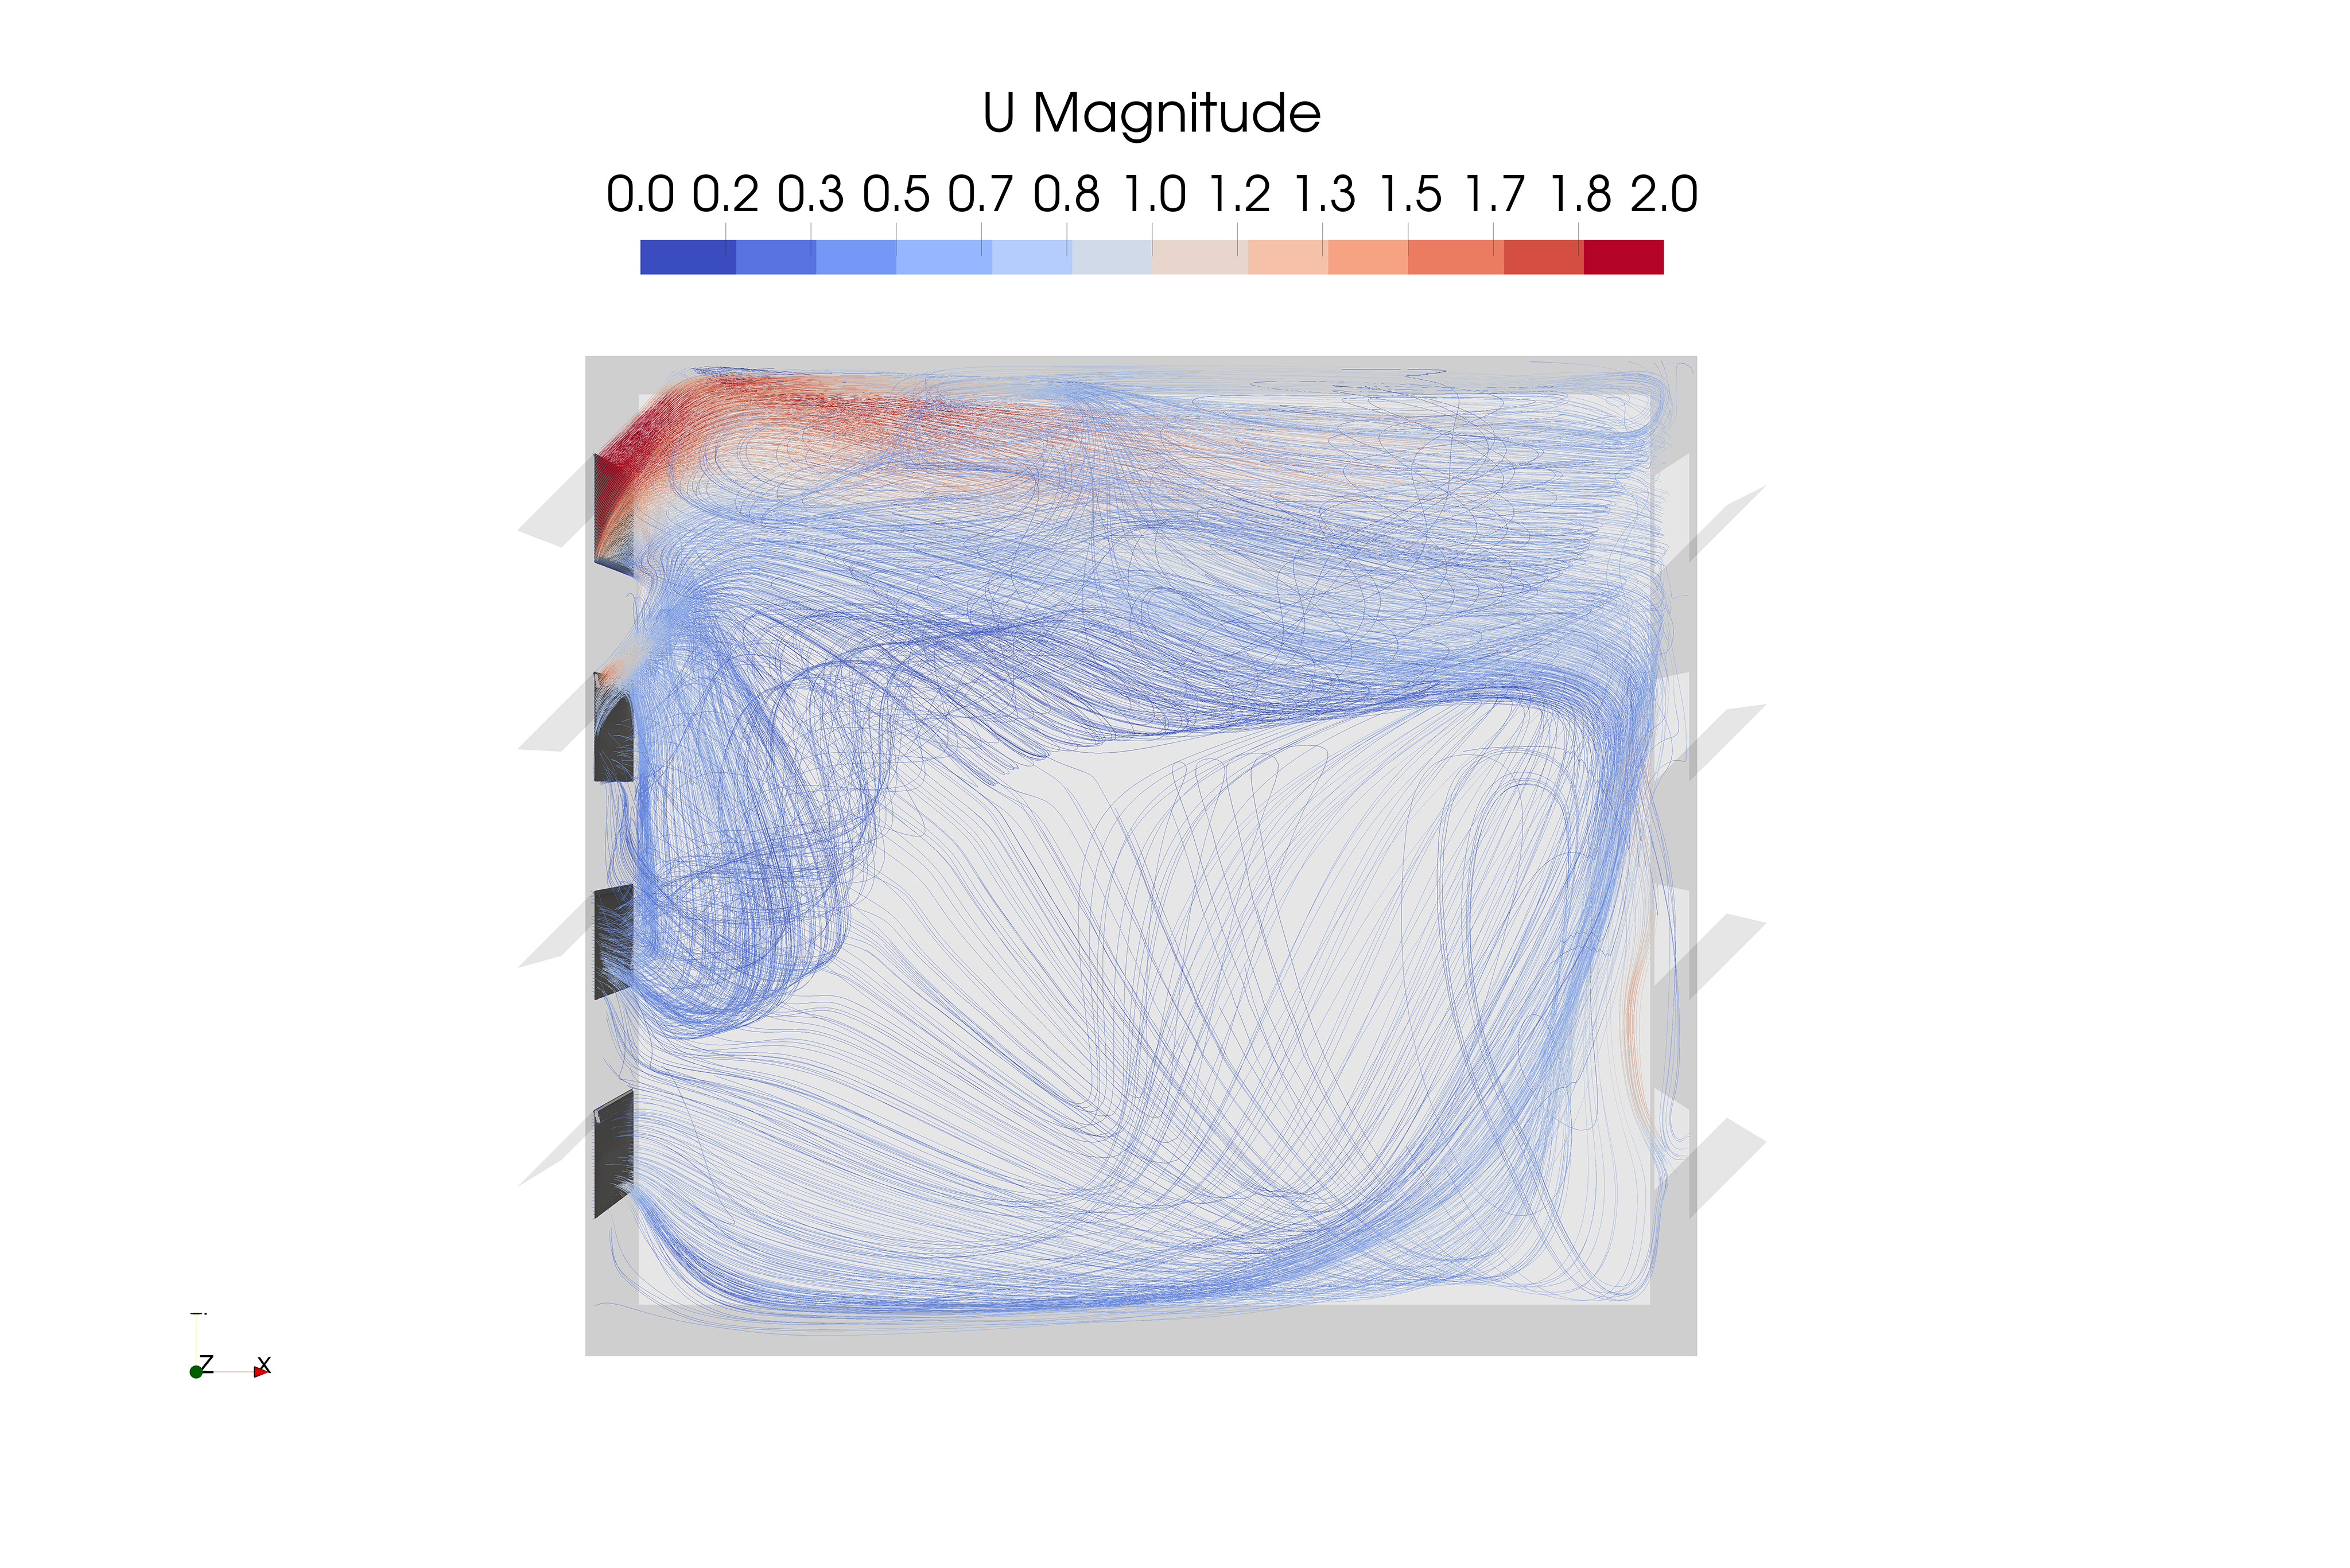
\includegraphics[width=.33\textwidth, trim= 31cm 12.5cm 35cm 17.5cm, clip]{images/AoA/topview_streamlines_40m_magU_left.png}}\hfil	
	
	%	\subfloat[][0.25 m]%
	%	{\includegraphics[width=.33\textwidth, trim= 72cm 30cm 77cm 50cm, clip]{images/AoA/topview_Aoa_025m}}\hfil
	\subfloat[][]%
	{\includegraphics[width=.33\textwidth, trim= 36cm 15cm 36.5cm 25cm, clip]{images/AoA/topview_Aoa_05m}}\hfil
	%	\subfloat[][1 m]%
	%	{\includegraphics[width=.33\textwidth, trim= 72cm 30cm 77cm 50cm, clip]{images/AoA/topview_Aoa_1m}}\hfil
	\subfloat[][]%
	{\includegraphics[width=.33\textwidth, trim= 36cm 15cm 36.5cm 25cm, clip]{images/AoA/topview_Aoa_1_5m}}\hfil
	%	\subfloat[][RNGkeps]%
	%	{\includegraphics[width=.33\textwidth, trim= 72cm 30cm 77cm 50cm, clip]{images/AoA/topview_Aoa_1_75m}}\hfil
	%	\subfloat[][2 m]%
	%	{\includegraphics[width=.33\textwidth, trim= 72cm 30cm 77cm 50cm, clip]{images/AoA/topview_Aoa_2m}}\hfil	
	\subfloat[][]%
	{\includegraphics[width=.33\textwidth, trim= 36cm 15cm 36.5cm 25cm, clip]{images/AoA/topview_Aoa_2_5m}}\hfil	\\
	%		\subfloat[][0.5 m]%
	%	{\includegraphics[width=.33\textwidth, trim= 72cm 30cm 77cm 50cm, clip]{images/AoA/sideview_Aoa_3m.png}}\hfil
	%	\subfloat[][1 m]%
	%	{\includegraphics[width=.33\textwidth, trim= 72cm 30cm 77cm 50cm, clip]{images/AoA/sideview_Aoa_-1m.png}}\hfil
	%	\subfloat[][1 m]%
	%	{\includegraphics[width=.33\textwidth, trim= 72cm 30cm 77cm 50cm, clip]{images/AoA/sideview_Aoa_-3m.png}}\hfil
	
	
	%	\subfloat[][0.5 m]{\begin{tabular}[b]{c}
	%	%\includegraphics[width=.33\textwidth, trim= 72cm 70cm 77cm 70cm, clip]{images/AoA/sideview_plane_Aoa_3m}\\
	%	\includegraphics[width=.33\textwidth, trim=  72cm 70cm 77cm 70cm, clip]{images/AoA/sideview_plane_Aoa_1m}\\
	%	\includegraphics[width=.33\textwidth, trim=  72cm 70cm 77cm 70cm, clip]{images/AoA/sideview_plane_Aoa_-1m}\\
	%	\includegraphics[width=.33\textwidth, trim=  72cm 70cm 77cm 70cm, clip]{images/AoA/sideview_plane_Aoa_-3m}
	%	\end{tabular}}
	
	%	\subfloat[][2.5 m]%
	%	{\includegraphics[width=.30\textwidth, trim= 72cm 70cm 77cm 70cm, clip]{images/AoA/sideview_plane_Aoa_1m}}\hfil	
	%	\subfloat[][2.5 m]%
	%	{\includegraphics[width=.30\textwidth, trim=72cm 70cm 77cm 70cm, clip]{images/AoA/sideview_plane_Aoa_-1m}}\hfil	
	%	\subfloat[][2.5 m]%
	%	{\includegraphics[width=.30\textwidth, trim= 72cm 70cm 77cm 70cm, clip]{images/AoA/sideview_plane_Aoa_-3m}}\hfil	
	\vspace*{0.4cm}
	\includegraphics[scale=.06, trim= 72cm 160cm 65cm 20cm, clip]{images/AoA/scale_AoA}
	\centering
	\subfloat[][]%
	{\hspace*{2cm}\includegraphics[width=.7\textwidth, trim= 31cm 20.5cm 35cm 40.5cm, clip, angle= 2]{images/AoA/pers_Plume_Aoa_100s_slice_1_5m_2.png}}\hfil	
	\captionsetup{format=plain}
	\caption[Local age of air in comparison to other visualisations methods of flow properties in a room.]{Local age of air in comparison to other visualizations methods of flow properties in a room. \textbf{(a)} Geometry with \SI{2.7}{\metre} ceiling height. \textbf{(b)} Horizontal cross-section at \SI{1}{\metre} colored by  $|u|$. \textbf{(c)} Horizontal cross-section at \SI{1}{\metre} showing vectors of $|u|$. \textbf{(d-f)} \num{10}, \num{20} and \SI{40}{\metre} of velocity streamlines passing the left facade colored by $|u|$.  \textbf{(g-i)} Horizontal cross-section of local age of air in \si{\second} at $z =$ \num{0.5}, \num{1.5} and \SI{2.5}{\metre}. \textbf{(j)} Streamlines colored and age of air combined.}
	\label{fig:Age_of_air_single_classroom}
\end{figure}







%\newpage
\section{Summary}
\enlargethispage*{2cm}
This chapter presented three ventilation metrics that have been successfully implemented in \OF. 
The three metrics may be distinguished with regard to their applicability and effort required to implement and post-process them.

\begin{enumerate}
	\item \blindtext[1]	
	
	
	
	\item \blindtext[1]	
	
	
\end{enumerate}
\enlargethispage*{2cm}
A visual comparison of the three implemented metrics is provided in \fref{fig:ACR_ventilation_metrics_comparison}. Shown is a horizontal cross-section through a building for an inlet velocity of \SI{1}{\metre\per\second} in negative y-direction.

